\chapter{Technologien}\label{chap:technologies}

Die richtige Technologie zur Lösung einer Problemstellung auszuwählen garantiert noch keinen Erfolg, ist aber ein wichtiger Grundstein um überhaupt erfolgreich sein zu können. In diesem Sinne sollte nicht zu wenig Augenmerk auf den Vergleich und die Entscheidung zwischen auf dem Markt verfügbaren Alternativen gelegt werden. Dieses Kapitel beschreibt, welche Technologien für welchen Teil der Architektur in Frage kommen, stellt diese gegenüber und begründet die Entscheidung für die am besten geeignetste Alternative.

\section{Entwicklungsumgebung}
Die Entwicklung des \nameformat{\gls{crm}} findet momentan ausschließlich mit \nameformat{Microsoft Visual Studio} statt. Wie in Kapitel~\ref{chap:requirements} ist gibt es die Core-Komponente und Desktopkomponente, welche in C++ geschrieben sind, und eine auf den Core aufsetzende, in C\# geschrieben, .NET-Komponente zur Bereitstellung der Webfunktionalität. Der bestehende Entwicklungsprozess soll nicht verändert und auch nicht weiter thematisiert werden, da die neu zu entwickelnde UI-Schicht eine unabhängige Codebasis besitzt und auch konzeptionell von den bisherigen Schichten getrennt ist. 

Für das in Kapitel~\ref{chap:requirements} angesprochene Tool zum Einlesen und Konvertieren der bisherigen UI-Repräsentation wurde wegen der vorhandenen internen Infrastruktur ebenfalls Visual Studio verwendet. Die Wahl der Programmiersprache fiel auf C\#, da der Zugriff auf das Dateisystem und speziell auf XML-Dateien, das Format der momentanen Repräsentation, sehr einfach ist. 

Für die neu entstehenden Webtechnologien kann jeder beliebige Texteditor benutzt werden, da keine speziellen Funktionen einer IDE oder eines Editors notwendig sind. Der in den nachfolgenden Kapiteln entwickelte Code wurde aufgrund der guten Autovervollständigung, der Integration mit Versionsverwaltungstools und der einfachen Erweiterbarkeit, mit \nameformat{Visual Studio Code} von \nameformat{Microsoft} erstellt. Wichtiger als der Editor ist die Sprache für welche er benutzt wird. Im Bereich der Webentwicklung hat sich JavaScript ohne Konkurrenz durchgesetzt und ist die einzige Sprache, die von allen Browsern unterstützt wird. Das spiegelt sich auch in der Auswahl der Frontend-Frameworks wieder, welche alle entweder direkt oder indirekt in JavaScript geschrieben sind.   

\section{Frontend-Frameworks}
\subsection{Traditionelle Lösungen}
Frameworks und Bibliotheken die versuchen Entwicklern das Erstellen von UIs zu erleichtern gibt es schon sehr lange und in einer sehr großen Anzahl. Traditionelle Projekte wie jQuery-UI (Mobile), Bootstrap und neuere Namen (Materialize, Semantic-UI, Pure, etc.) setzen auf die Gestaltung von fertigen Komponenten die per CSS-Klasse in eine vorhandene Webseite integriert werden können. Durch diesen Fokus auf pures Styling mit CSS sind diese Projekte meist sehr klein und können schnell integriert werden. Sie eignen sich damit für rapides Prototyping, jedoch nicht um komplette Webseiten von Grund auf zu erstellen --- vielmehr können sie mit den unten angesprochenen JavaScript-Projekten im Zusammenspiel benutzt werden.

\subsection{Moderne, JavaScript-basierte Lösungen}
In jüngster Zeit haben komponentenbasierte Frameworks, Single-Page-Applications und Shadow-DOM starken Wachstum zu verzeichnen. \fixme{erklärung}
Auch in diesem Bereich gibt es sehr viel Auswahl, aufgrund der zeitlichen Limitierung werden jedoch nur die größten drei Mitstreiter \nameformat{Vue}, \nameformat{React} und \nameformat{Angular} \fixme{quelle, npm stats oder jahresrückblick} miteinander verglichen. Weitere Möglichkeiten für spätere Analysen sind \nameformat{Polymer}, \nameformat{Ember}, \nameformat{Knockout}, \nameformat{Riot}, etc.

\subsection{Vergleich Vue, React \& Angular}

\subsubsection{Generell}
\begin{itemize}
    \item{Vue}
    \item[] Entwickler legen viel Wert darauf möglichst kleine und dennoch performante Laufzeit zu entwickeln. Der Einstieg in \nameformat{Vue} soll möglichst einfach sein, was durch eine sehr gute Dokumentation und ein hervorragendes CLI-Tool zum Erstellen neuer Projekte gelingt. Abhängigkeiten zwischen Daten und UI verfolgt Vue selbstständig, es werden daher immer nur Elemente aktualisiert wenn sich auch deren anzuzeigende Daten geändert haben. Das Erstellen von nativen Apps ist bei \nameformat{Vue} nur mit Software von Drittherstellern möglich, die Entwickler arbeiten mit diesen aber zusammen um den Prozess zu verbessern. Das Verwenden von JavaScript-Templates (JSX) und \nameformat{Typescript} ist mit etwas Konfiguration ebenfalls möglich. \nameformat{Vue} hat im Vergleich noch ein kleines Ökosystem, kann aber dafür den stärksten Wachstum aller Frameworks verzeichnen.
    \item{React}
    \item[] \nameformat{React} diktiert im Vergleich zu \nameformat{Vue} noch weniger Vorgaben an die Entwickler, alle typischen Problemstellungen werden durch Bibliotheken gelöst. Dies ist möglich, da das Ökosystem sehr groß ist und eine breite und tiefe Auswahl an entsprechenden Bibliotheken bietet. Native Apps können mit dem vom gleichen Team entwickelten \nameformat{React-Native} erstellt werden ohne dafür weitere Software zu benötigen. Durch die Konzentration auf wesentliche Features und Verbesserungen und eine stabile API stellt das \nameformat{React}-Team sicher, dass Upgrades auf neue Versionen gar keine bis wenige Änderungen am bestehenden Code verlangen. Auch \nameformat{Typescript}-Integration und damit verbundenes Tooling (Linter, Type checks, Autocompletion) sind problemlos möglich.
    \item{Angular}
    \item[] Es werden für alle typischen Anforderungen die bei der Entwicklung anfallen bereits Tools und Konzepte mit ausgeliefert, um diese Anforderungen zu erfüllen. Dadurch ist \nameformat{Angular} an sich sehr viel mächtiger als \nameformat{Vue} und \nameformat{React}. Die Chance dafür dass man abgesehen von \nameformat{Angular} noch weitere große Bibliotheken benötigt ist gering, jedoch erfordert die Nutzung dieser mitgelieferten Möglichkeiten auch dass man sie gut genug kennt. Der Einstieg in \nameformat{Angular} wird von vielen daher als mühsam und zeitintensiv beschrieben. Die Dokumentation ist sehr umfangreich, teilweise aber auch unübersichtlich und das Ökosystem von \nameformat{Angular} ist zwar größer als das von \nameformat{Vue}, es hat jedoch auch negatives Wachstum zu verzeichnen.
\end{itemize}

\subsubsection{Aufbau von Apps (mit Beispielkomponente)}
Um zumindest ein Gefühl für das Benutzen der jeweiligen Frameworks zu bekommen wurde eine Beispielkomponente ausgewählt die mit allen drei Frameworks umgesetzt werden soll. In Abbildung~\ref{fig:example_component} sieht man die fertige Komponente. Bei Klick in das Edit-Feld ändert sich die Farbe des Randes um den Fokus zu signalisieren. Ändert man den Eintrag kann diese Änderung mit Escape verworfen oder mit Enter gespeichert werden. Der Text darunter gibt immer den momentan gespeicherten Wert wieder. Die Komponente wurde in Online-Editoren erstellt welche bereits eine fertig Umgebung mit dem jeweiligen Framework bieten. Auf die Benutzung weiterer Bibliotheken wurde hier explizit verzichtet.

\begin{figure}
    \centering
    \captionsetup{justification=centering}
    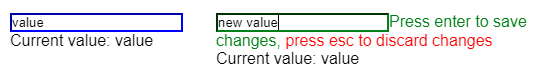
\includegraphics{figures/example_component.png}
        \caption{Beispielkomponente für die Umsetzung mit allen Frameworks}\label{fig:example_component}
\end{figure}


\begin{itemize}
    \captionsetup{justification=centering}
    \item{Vue}
    \item[] Die \nameformat{Vue}-Komponente wird komplett als Instanz einer \nameformat{Vue}-Klasse angelegt, der man Daten und Methoden übergeben muss. Im HTML-Template werden die \nameformat{Vue}-eigenen Attribute ersichtlich.
    \item[] \lstinputlisting[language={JavaScript}, label={lst:vue_example},caption={Umsetzung der Beispielkomponente mit Vue}]{code/chapter_003_vue_example.js}
    \item{React}
    \item[] Eine \nameformat{React}-Komponente kann entweder als herkömmliche Klasse oder nur als Funktion, welche die darzustellenden UI-Elemente als Rückgabewert enthält, angegeben werden.
    \item[] \lstinputlisting[language={JavaScript}, label={lst:react_example},caption={Umsetzung der Beispielkomponente mit React}]{code/chapter_003_react_example.js}
    \item[] \lstinputlisting[language={JavaScript}, label={lst:react_hooks_example},caption={Funktionale Umsetzung der Beispielkomponente mit React}]{code/chapter_003_react_hooks_example.js}
    \item{Angular}
    \item[] Bei \nameformat{Angular} besteht eine Komponente wie bei \nameformat{React} aus einer herkömmlichen Klasse. Diese wird jedoch mit einer speziellen Annotation mit Informationen über das Aussehen und die Platzierung der Komponente versehen.
    \item[] \lstinputlisting[language={JavaScript}, label={lst:angular_example},caption={Umsetzung der Beispielkomponente mit Angular}]{code/chapter_003_angular_example.js}
\end{itemize}

\subsubsection{State-Management}
\begin{itemize}
    \item{Vue}
    \item[] Standard ist, dass jede Komponente ihr eigenes State-Objekt besitzt. Zusätzlich dazu kann noch auf das State-Objekt der \nameformat{Vue}-Instanz in der sich die Komponente befindet (Parent) zugegriffen werden. Dieses kann entweder direkt verändert oder per Store-Pattern \fixme{footnote?} verwaltet werden. \nameformat{Vuex} ist eine direkt von \nameformat{Vue} entwickelte Bibliothek welche das genannte Store-Pattern umsetzt.
    \item{React}
    \item[] \nameformat{React} unterstützt nur einen unidirektionalen Datenfluss mit ``Props''. Diese werden Komponenten von ihren Elternkomponenten mitgegeben. Jede Komponente hat ihren eigenen State der per Props an Kinder weitergegeben (aber nicht direkt verändert) werden kann. Es gibt einige bekannte Bibliotheken welche das Verwaltung von State auf andere Arten lösen. \nameformat{Redux} setzt das funktionale Flux-Pattern um, dabei werden Änderungen per Aktions-Event ausgelöst, die Events von Reducern ausgewertet und der State entsprechend verändert. Der neue State wird den entsprechenden UI-Elementen wieder unveränderbar (immutable) übergeben. \nameformat{MobX} und \nameformat{react-easy-state} setzen das bei \nameformat{Vue} erwähnte Store-Pattern in \nameformat{React} um.
    \item{Angular}
    \item[] State wird direkt in den Klasseninstanzen der Komponenten gespeichert und kann durch herkömmliche OOP-Konzepte weitergegeben und verändert werden. Zusätzlich existiert auch \nameformat{NGXS}, welches auf dem gleichen Prinzip wie \nameformat{Redux} beruht, aufgrund moderner \nameformat{Typescript}-Features laut \nameformat{Angular} aber einfacher zu benutzen sei.
\end{itemize}

\subsubsection{Routing}
\begin{itemize}
    \item{Vue}
    \item[] Routing ist direkt in \nameformat{Vue} integriert. Routen werden in JavaScript mit Komponenten verknüpft und bei Aufruf dieser Route wird die verknüpfte Komponente an einen zuvor festgelegten Platzhalter im DOM gerendert.
    \item{React}
    \item[] Nicht integriert, es gibt aber mehrere Alternativen als Bibliotheken. Bei \nameformat{Aviator} werden Routen als geschachteltes Objekt übergeben, bei dem jedes Element eine Route und eine Zielfunktion enthält. Die Zielfunktion wird aufgerufen wenn zur entsprechenden Route navigiert wird und muss wissen wie und wohin (etwa über Dokument-Selektoren) die entsprechende Komponente gerendert werden muss. Die Nutzung von JSX ist dabei nicht mehr möglich. Bei \nameformat{react-router} hingegen werden die Routen deklarativ in den JSX-Templates hinterlegt. Sie enthalten als Property die Route für die sie gerendert werden sollen und die eigentliche Komponente die angezeigt werden soll.
    \item{Angular}
    \item[] Analog zu \nameformat{Vue} ist auch hier eine Lösung direkt integriert und funktioniert auch nach dem exakt gleichen Prinzip.
\end{itemize}

\subsubsection{Testing}
\begin{itemize}
    \item{Vue}
    \item[] \nameformat{Vue} enthält Test-Tools mit denen man Komponenten in Variablen rendern kann. Diese gespeicherten Komponenten sind herkömmliche JavaScript-Objekte und können dann mit weiteren (externen) Tools auf bestimmte Zustände und Eigenschaften geprüft werden.
    \item{React}
    \item[] Das Testen von \nameformat{React}-Komponenten funktioniert analog zu \nameformat{Vue}.
    \item{Angular}
    \item[] Alle zum Testen benötigten Tools sind bereits enthalten und sehr ausführlich dokumentiert. Wenn nur bestimmte Teilaspekte einer Anwendung wie etwa die UI-Komponenten getestet werden sollen ist der Aufwand dies einzurichten durch die Notwendigkeit sich mit dem kompletten Test-Konzept auseinander setzen zu müssen höher als bei \nameformat{Vue} und \nameformat{React}.
\end{itemize}

\subsubsection{\acrlong{ssr}}
Bei allen Frameworks gibt es auch die Möglichkeit nur wenige Seiten ``vor-gerendert'' auf dem Server liegen zu haben anstatt sie dynamisch bei entsprechenden Anfragen zu generieren. Hierfür kann das \nameformat{Node.js} Tool \nameformat{Prerender.io} benutzt werden.
\begin{itemize}
    \item{Vue}
    \item[] \nameformat{Vue} liefert einen dafür vorgesehenen Renderer (\nameformat{vue-server-renderer}) der Markup als Text generiert. Das kann beim initialen Laden der Seite ausgeliefert werden (erfordert einen \nameformat{Node.js} Server).
    \item{React}
    \item[] Auch \nameformat{React} liefert einen dafür vorgesehenen Renderer (\nameformat{ReactDOMServer}) der Markup als Text generiert. Das kann beim initialen Laden der Seite ausgeliefert und auf Clientseite mit ReactDom.hydrate() mit Inhalten gefüllt werden (erfordert einen \nameformat{Node.js} Server).
    \item{Angular}
    \item[] \nameformat{Angular} benötigt für \gls{ssr} zusätzliche Abhängigkeiten, Änderungen an der Konfiguration, ein zusätzliches Build / Bundle Target und ein zusätzliches Modul mit extra Konfiguration das auf dem Server läuft und dafür zuständig ist das neue JS-Bundle auszuliefern.
\end{itemize}

\subsection{Fazit}
Alle betrachteten Alternativen sind valide Optionen mit denen jegliche Anforderungen umgesetzt werden können. Der Einstieg in \nameformat{Angular} scheint allerdings schwierig, da dort eine Vielzahl an Technologien für verschiedenste Zwecke mitgeliefert werden. Da es seitens der Funktionalität kein Unterschiede gibt kommt es mehr oder weniger darauf an welches Projekt einem Entwickler (-team) am meisten zusagt bzw.\ mit welchem es am besten arbeiten kann.
\nameformat{React} besitzt mit Abstand die größte Community, es kann daher davon ausgegangen werden, dass die Weiterentwicklung, viele aufsetzende Bibliotheken und Ressourcen im Netz garantiert sind. Ein weiterer Vorteil, die Benutzung von \nameformat{Typescript} vorausgesetzt, ist die IDE-Unterstützung beim Schreiben der Komponenten-Templates. Im Vergleich zu \nameformat{Vue} wird bei \nameformat{React} hier ausschließlich JavaScript genutzt, was es erlaubt die Typisierung von \nameformat{Typescript} zu nutzen um Autovervollständigung oder ähnliche Hilfen anzuwenden. \nameformat{Vue} hingegen schreibt JavaScript-Funktionsaufrufe in Strings und nutzt eigene, für nicht \nameformat{Vue}-Entwickler unbekannte, HTML-Attribute für Schleifen und Verzweigungen --- da es sich dabei um \nameformat{Vue}-Sonderfälle handelt kann die IDE oft nicht helfen, es liegt also am Entwickler das entsprechende Wissen aufzubauen und keine Fehler zu machen.

Für den Prototypen wird vorerst \nameformat{React} genutzt. Da die die Technologien zur Laufzeit alle kompatibel sind (sie werden alle in normales HTML, CSS und JavaScript transpiliert), kann dieser Code später aber auch mit Vue zusammen genutzt oder nach und nach ersetzt werden.

\section{TypeScript}
Bei JavaScript handelt es sich um eine dynamisch typisierte Sprache, dass heißt das sich Typen von Variablen zur Laufzeit ändern können und vor der Nutzung einer Variablen entsprechend überprüft werden müssen. Dies ist ein Vorteil wenn schnell kleinere Skripte geschrieben werden bei denen aufgrund ihrer überschaubaren Größe entsprechende Überprüfungen trivial sind oder es schlichtweg keine Rolle spielt ob ein Skript Fehler enthält. Für die Entwicklung von größeren Projekten ist diese Eigenschaft jedoch ein gravierender Nachteil, da Typen von Variablen im Code durch Entfernung von Deklaration und Nutzung nicht ersichtlich sind und daraus resultierende Fehler bei der Benutzung immer erst zur Laufzeit der betroffenen Zeilen auftreten oder sogar gar nicht als Fehler erkennbar sind und lediglich ein falsches (aber nicht unbedingt als falsch erkennbares) Ergebnis liefern.   

Um dieser Art von subtilen Bugs vorzubeugen bietet \nameformat{Microsoft} seit 2012 \nameformat{TypeScript} an. Es handelt sich dabei um eine typisierte open-source Sprache welche als syntaktische Obermenge von JavaScript (normaler JavaScript-Code ist also ebenso gültiger \nameformat{TypeScript}-Code) beschrieben werden kann und die zu gewöhnlichem JavaScript transpiliert\footnote{Übersetzung von Quellcode aus einer Programmiersprache in eine andere} wird und somit trotz ihrer Vorteile keinen Kompatibilitätsnachteil besitzt. Da die Syntax auf JavaScript basiert ist das Erlernen dieser für JavaScript-Entwickler trivial. Durch Nutzung von typisierten Daten werden fehlerhafte Nutzungen von Variablen bereits bei der Entwicklung, eine entsprechende Integration des Editors vorausgesetzt, oder spätestens beim Transpilieren bemerkt und dem Entwickler als solche angezeigt. Ebenso erlaubt eine Editorintegration das Anbieten von Codevervollständigung und damit zu einem effektiveren Entwicklungsprozess.

Der einzige Nachteil von \nameformat{TypeScript} ist, dass ein zusätzlicher Schritt zum Übersetzen in JavaScript-Code notwendig ist. Da die meisten Projekte im Webbereich aber sowieso nicht komplett ohne ähnliche Tooling-Schritte auskommen und der \nameformat{TypeScript}-Compiler einfach in diese bestehenden Prozesse integrierbar ist handelt es sich hierbei nur um eine überschaubare Einschränkung. Dieser Nachteil kann aber auch positiv ausgelegt werden, da es durch den Übersetzungsschritt möglich ist, bereits Features und Standards zu benutzen, welche noch nicht von allen Browsern unterstützt werden. Bei der Übersetzung werden diese in semantisch identischen Code umgewandelt, der unter Einhaltung von älteren Standards gültig ist, aber für den Entwickler schwieriger zu schreiben wäre. 

Aufgrund dieser Argumentation soll zur Unterstützung der Entwickler und Vorbeugen von Fehlern bei die Entwicklung der \nameformat{React}-Seite ausschließlich \nameformat{TypeScript} benutzt werden. 

\section{API-Anbindung}
Die Anbindung der API kommen zwei Ansätze in Frage: \nameformat{Rest} und \nameformat{GraphQL}\@. Bei \nameformat{Rest} handelt es sich um einen Architekturstil bei dem Ressourcen über URI-Endpunkte angesprochen und abgerufen werden. \nameformat{GraphQL} hingegen ist eine von \nameformat{Facebook} entwickelte Query-Sprache zur Abfrage von vorhandenen Daten. In diesem Abschnitt werden speziell die für dieses Projekt relevanten Vor- und Nachteile beider Ansätze angesprochen.

\subsection{Rest}
\nameformat{Rest}-APIs sind heutzutage die Norm, um die Architektur allerdings korrekt umzusetzen ist aber mit viel Arbeit und gewissen Nachteilen verbunden. Dies könnte einer der Gründe dafür sein, dass ein großer Teil der angesprochenen \nameformat{Rest}-APIs nur ``Rest-like'' sind. Als ``Rest-like'' werden die Implementationen bezeichnet, welche das sogenannte HATEOAS~\footnote{Hypermedia as the Engine of Application State}-Konzept nicht umsetzen. Das Konzept beschreibt, wie ein Client durch die API navigieren soll --- alle validen Übergänge vom momentanen State in den nächsten sind bereits in der momentanen Antwort einer Anfrage in Form von Links und Metadaten verfügbar. Ein Konsument muss damit nicht mehr wissen, welche Anfragen zu welchem Zeitpunkt gültig sind und kann immer genau die Aktionen anbieten, die auch von der API angeboten werden. Eine Versionierung der API (und damit stärkere Kopplung von Clients und Server) entfällt ebenfalls, neue Features können als weitere Aktion-Links auftauchen und alte Features zusätzlich zu einem Link die Information erhalten, dass die Aktion bald nicht mehr zur Verfügung stehen wird. Trotz verschiedener Standards die beim Erstellen der Struktur der Daten, vor allem bezgl.\ der Metadaten und wie diese ausgelesen werden können, helfen, ist es aufgrund des Mehraufwands bei jedem Endpoint dennoch mühsam eine \nameformat{Rest}-API mit HATEOAS korrekt zu implementieren. Zusätzlich dazu, und dieser Nachteil wird im Gegenzug zu der gerade beschriebenen Flexibilität absichtlich in Kauf genommen, können solche APIs nur navigiert werden, indem vielen Links gefolgt und damit viele Netzwerkanfragen gemacht werden. 
Die Alternative, \nameformat{Rest}-APIs ohne HATEOAS zu erstellen, ist zwar für die Entwickler einfacher, das Konsumieren der API wird dadurch aber deutlich erschwert. Eine Anbindung ist nur möglich indem dauerhaft die Dokumentation (welche in entsprechender Qualität vorhanden sein muss) konsultiert wird. Bei Änderungen an der API müssen auch die Clients angepasst werden, da sie keine Möglichkeit haben die Änderungen direkt mit zu bekommen.
Um die Erstellung von richtigen \nameformat{Rest}-APIs zu vereinfachen gibt es den \nameformat{OData}-Standard der Entwicklern unter anderem die Definition und die Erstellung von Metadaten abnimmt, sodass diese sich auf die eigentliche Programmlogik konzentrieren können.

Caching ist bei \nameformat{Rest} einfacher möglich als bei \nameformat{GraphQL}, da jedes Endpoint-Daten-Paar als ein Eintrag im Cache angesehen werden kann. Werden entsprechende Cache-Header in den HTTP-Nachrichten gesetzt werden die Daten vom Browser (und eventuell vorhandenen Cache-Proxies) automatisch verwaltet. Dies funktioniert, weil Anfragen einer Ressource bei Rest immer alle Daten erhalten, die es zu dieser Ressource gibt. Um nicht immer alle Daten übertragen zu müssen besitzen viele \nameformat{Rest}-APIs Parameter, mit denen man eine Anfrage einschränken kann. Je granularer diese Einschränkungen sind desto weniger überflüssige Daten müssen übertragen werden, gleichzeitig greift damit aber auch der Cache immer seltener, weil dauerhaft andere Endpoint-Daten-Paare angefragt werden.

\subsection{GraphQL}
Einer der Hauptgründe für die Entwicklung von \nameformat{GraphQL} ist die höhere Netzwerklast bei \nameformat{Rest}-APIs, die insbesondere bei mobilen Clients sehr negativ auffallen kann. Ein Hauptaugenmerk der Technologie ist deswegen, in diesem Bereich möglichst sparsam zu sein und möglichst wenig Daten zu übertragen.
\nameformat{GraphQL} ist laut npm \fixme{quelle} die im Webbereich am meisten wachsende Technologie überhaupt, als Folge dessen wird es in Zukunft wahrscheinlich in vielen Projekten benutzt werden, der Aufbau von entsprechendem Know-How in diesem Bereich ist daher wichtig.
Eine Abfrage bei \nameformat{GraphQL} hat den gleichen Aufbau wie ein JSON-Dokument, mit der Besonderheit dass anstatt Schlüssel-Werte-Paaren nur Schlüssel bzw. der Name von Ressourcen angegeben werden. Eine Antwort hat immer den gleichen Aufbau wie eine Anfrage, die Schlüssel bzw. Ressourcennamen werden dabei wie in Listing~\ref{lst:graphql_example_query} zu sehen mit den ausgelesenen Daten ergänzt. Durch die Nutzung von Typen für diese Abfragen kann garantiert werden, dass eine von den Tools akzeptierte Anfrage auf jeden Fall ein Ergebnis vom Server liefern wird. Die Abfragen müssen dabei nicht alle Felder einer Ressource enthalten, es können immer genau die Daten abgefragt werden die in einer spezifischen Situation gerade benötigt werden. Ebenfalls können mehrere unabhängige Anfragen zu einer großen Anfrage zusammengefasst und mit nur einem HTTP-Roundtrip beantwortet werden.
Das typisierte Schema erlaubt weiterhin, Konsumenten jederzeit Informationen über sich selbst (Metadaten), etwa den Type eines Feldes oder weitere mögliche Felder zur Abfrage, zur Verfügung zu stellen. Vorausgesetzt ein Client kennt einen den Einsprungpunkt eines Graphen kann er mit diesen Metainformationen alle weiteren Informationen programmatisch auslesen. 

\lstinputlisting[language={JavaScript}, label={lst:graphql_example_query},caption={Beispielquery aus der GraphQL Dokumentation \fixme{quelle?}}]{code/chapter_003_graphql_example_query.js}

Um Entwickler zu unterstützen existiert ein visueller Query-Editor \nameformat{GraphiQL} mit Autovervollständigung und aus dem Schema generierter Dokumentation. Mithilfe diesen Editors kann sehr leicht in der API navigiert und direkt code-seitig benutzbare Abfragen generiert werden.
Viele moderne Webseiten basieren nicht mehr nur auf der Annahmen, dass irgendwann Daten vom Server abgefragt werden, sondern auch darauf dass serverseitige Events / Änderungen das Laden oder Anzeigen von Daten auslösen können. \nameformat{GraphQL} spezifiziert für diese Anforderung ein Abonnement-System: ein Client registriert sich beim Server für alle Daten, deren Änderung er sofort mitbekommen möchte und gibt an, welche Abfrage dafür ausgeführt werden soll. Bei einer Änderung wird diese Abfrage dann ausgeführt und die Daten über eine Websocket-Verbindung sofort an den Client übertragen.

Um diese ganzen Eigenschaften zu ermöglichen ist es jedoch notwendig, dass sowohl der Client als auch der Server mit dem gleichen \nameformat{GraphQL}-Schema arbeiten und damit aneinander gekoppelt sind.
Ein weiterer Nachteil ist es, dass Aufgrund der Nutzung von \nameformat{GraphQL} (nur HTTP-POST und identischer Endpoint) Caching nicht auf HTTP-Ebene geschehen kann und damit die Verantwortung für gute Cache-Strategien hauptsächlich beim Client liegen.

Zwei bekannte Bibliotheken welche die \nameformat{GraphQL}-Spezifikation in JavaScript umsetzen und das Erstellen von Queries, Caching und Debuggen erleichtern sind \nameformat{Apollo} und \nameformat{Relay}. \nameformat{Relay} wurde ebenfalls von \nameformat{Facebook} entwickelt, dennoch hat \nameformat{Apollo} eine sehr viel größere Community. Für die Umsetzung im Backend (.NET) existieren ebenfalls Implementierungen, die am meisten genutzte davon ist \nameformat{graphql-dotnet}.

\subsection{Fazit}

\nameformat{Rest} und \nameformat{GraphQL} können beide für den gleichen Zweck benutzt werden, sie konkurrieren jedoch nicht direkt miteinander. Eine API kann ebenso beide Ansätze entweder ergänzend oder parallel anbieten. Bestehende \nameformat{Rest}-APIs können durch das Resolver-Konzept von \nameformat{GraphQL} auf einfache Art und Weise gewrapped werden und so auf beide Arten angesprochen werden. \nameformat{Rest} ist flexibler als \nameformat{GraphQL}, um diese Flexibilität aber richtig zu nutzen und damit eine API zu schreiben welche viele Jahre genutzt und skaliert werden kann ist aber viel Erfahrung und Aufwand notwendig. \nameformat{GraphQL} scheint daher als die richtige Wahl für Firmen oder Personen die noch nicht viel Erfahrung in diesem Bereich sammeln konnten. \nameformat{GraphQL} benötigt sowohl eine Server als auch eine Clientkomponente und hat damit mehr Abhängigkeiten als dies bei \nameformat{Rest} der Fall ist, im Gegenzug ist es dadurch aber möglich effiziente, typsichere Anfragen zu erstellen. Ebenso wird mit dem mitgelieferten \nameformat{GraphiQL}-Tool ein Abfrage-Editor mit Autovervollständigung und Fehlerbeschreibungen bereitgestellt, der es Nutzern sehr einfach macht eine API und deren Möglichkeiten zu erkunden sowie für alle Bestandteile direkt eine Dokumentation einzusehen. Ein weiterer Vorteil von \nameformat{GraphQL} ist es, dass durch die typisierten Abfragen eine automatische Generierung von Mocking-Daten möglich ist. Mithilfe solcher Mocking-Daten kann das Entwicklerteam den API Client im Frontend entwickeln und testen, bevor das Backend mit den Echtdaten zur Verfügung steht.

Wegen der einfacheren Nutzung von \nameformat{GraphQL} und der besseren Unterstützung von Entwicklern durch Typisierung und mitgelieferten Tools wird im Prototyp diese Technologie verwendet.
